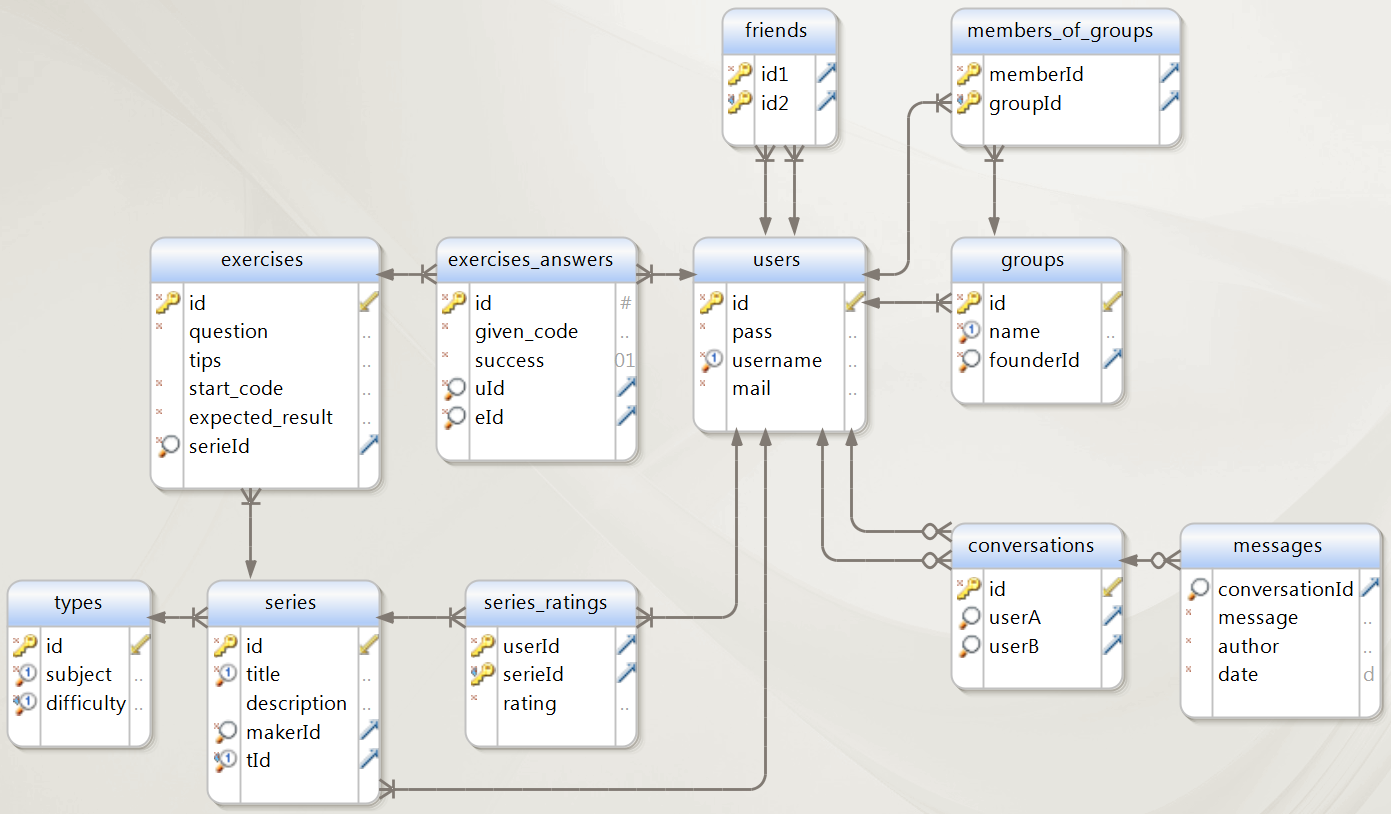
\includegraphics[keepaspectratio=true, angle=90, scale=0.33]{raport_files/design/UML}

\begin{itemize}
    \item \emph{Users} are one of the most important parts of the application. These are the members
        of the website. Only registered members are qualified as users, mere guests are not observed
        in any way.
    \item \emph{Friends} is a 1-to-1 relationship. In order te become friends, a request is sent and
        must be accepted.
    \item \emph{Groups} are collections of users. Each group has a founder and other Users can join 
        a group. No requests are necessary.
    \item \emph{Members of groups} are the users that form such a group. Each group contains at least 1 member
        this is the founder of the group.
    \item \emph{Converstations} are collections of messages between two users.
    \item \emph{Messages} are the content of a conversation.
    \item \emph{Series} are the second most import parts of the application (besides the Users). Each Series
        is a set of Exercises. A series also has a type and a rating.
    \item \emph{Series rating} are ratings given by users who have completed the series. This will
        be used to make recomendations to other users.
    \item \emph{Types} are a tuple of a subject and a difficulty. This tuple uniquely identifies each type.
    \item \emph{Exercises} are what makes a Series. It contains a question, tips for solving
        the exercise (optionally), start code to give the user a starting point and an expected result.
        This expected result is compared to the output generated by the interpreter.
    \item \emph{Exercises answers} are the updated code given in the exercise. The result of this code
        will be used to determine wether the answer yields the correct output.
\end{itemize}

